\section{Case Description and Requirement Elicitation}
\label{sec:requirement_elicitation}

In this chapter an overview will be given on the Case Study at hand. Alongside this description, light will be shed on the requirements to consider for further implementation and architectures.

\subsection{Case Description}
\label{subsec:case_description}

As covered in the previous sections of this project, Self-Sovereign Identity for IoT devices is a field which has yet to discover its full potential. Exploring the capabilities of SSI concepts in this field will allow further researchers to understand whether certain limitations of these environments caps the usage of DIDs, VCs and more SSI concepts. A field within the IoT scope which has seen an increase in demand in recent times, is the \glspl{EV} interactions. These type of interactions are included in a subset of the IoT devices, namely the IoV domain, which was already mentioned in Section~\ref{subsubsec:link_between_ssi_and_IoTIoV}.

The Case Study which will be the aim of this project is how to enable Self-Sovereign Identity within an EV Charging interaction, powered by Electric Vehicle Charging Stations. 

For the purpose of extracting information on the current architecture of the system, a domain expert was interviewed to assess the details of the current system, as well as to extract the requirements for a novel approach targeted for the same end. The following description of the system was developed over the span of several weeks and over a number of interactions with the expert, to match the details with the current reality of EV Charging.

A high-level overview of the system can be observed in Figure~\ref{fig:High-level overview}. In this diagram it is possible to see the involved parties as well as the types of communication some parties have between each other in the current system architecture. Alongside the diagram it is possible to see a legend with a description of the different parties.

The main goal of this work is to provide the benefits of Self-Sovereign Identity mentioned in Section~\ref{subsubsec:link_between_ssi_and_IoTIoV} into the Electric Vehicle Charging use case. Multiple parties will need to trust each other in order for an exchange of energy to take place. Making use of the Verifiable Credentials explained in Section~\ref{subsubsec:VCs} it is possible to guarantee that a vehicle belongs to a given owner, that the vehicle is itself, and several other claims which will be described later in this document.

More clarity will be given on the parties and their roles in the current system, and what types of communication occur in this system.

\begin{figure}[!htb]
    \centering
    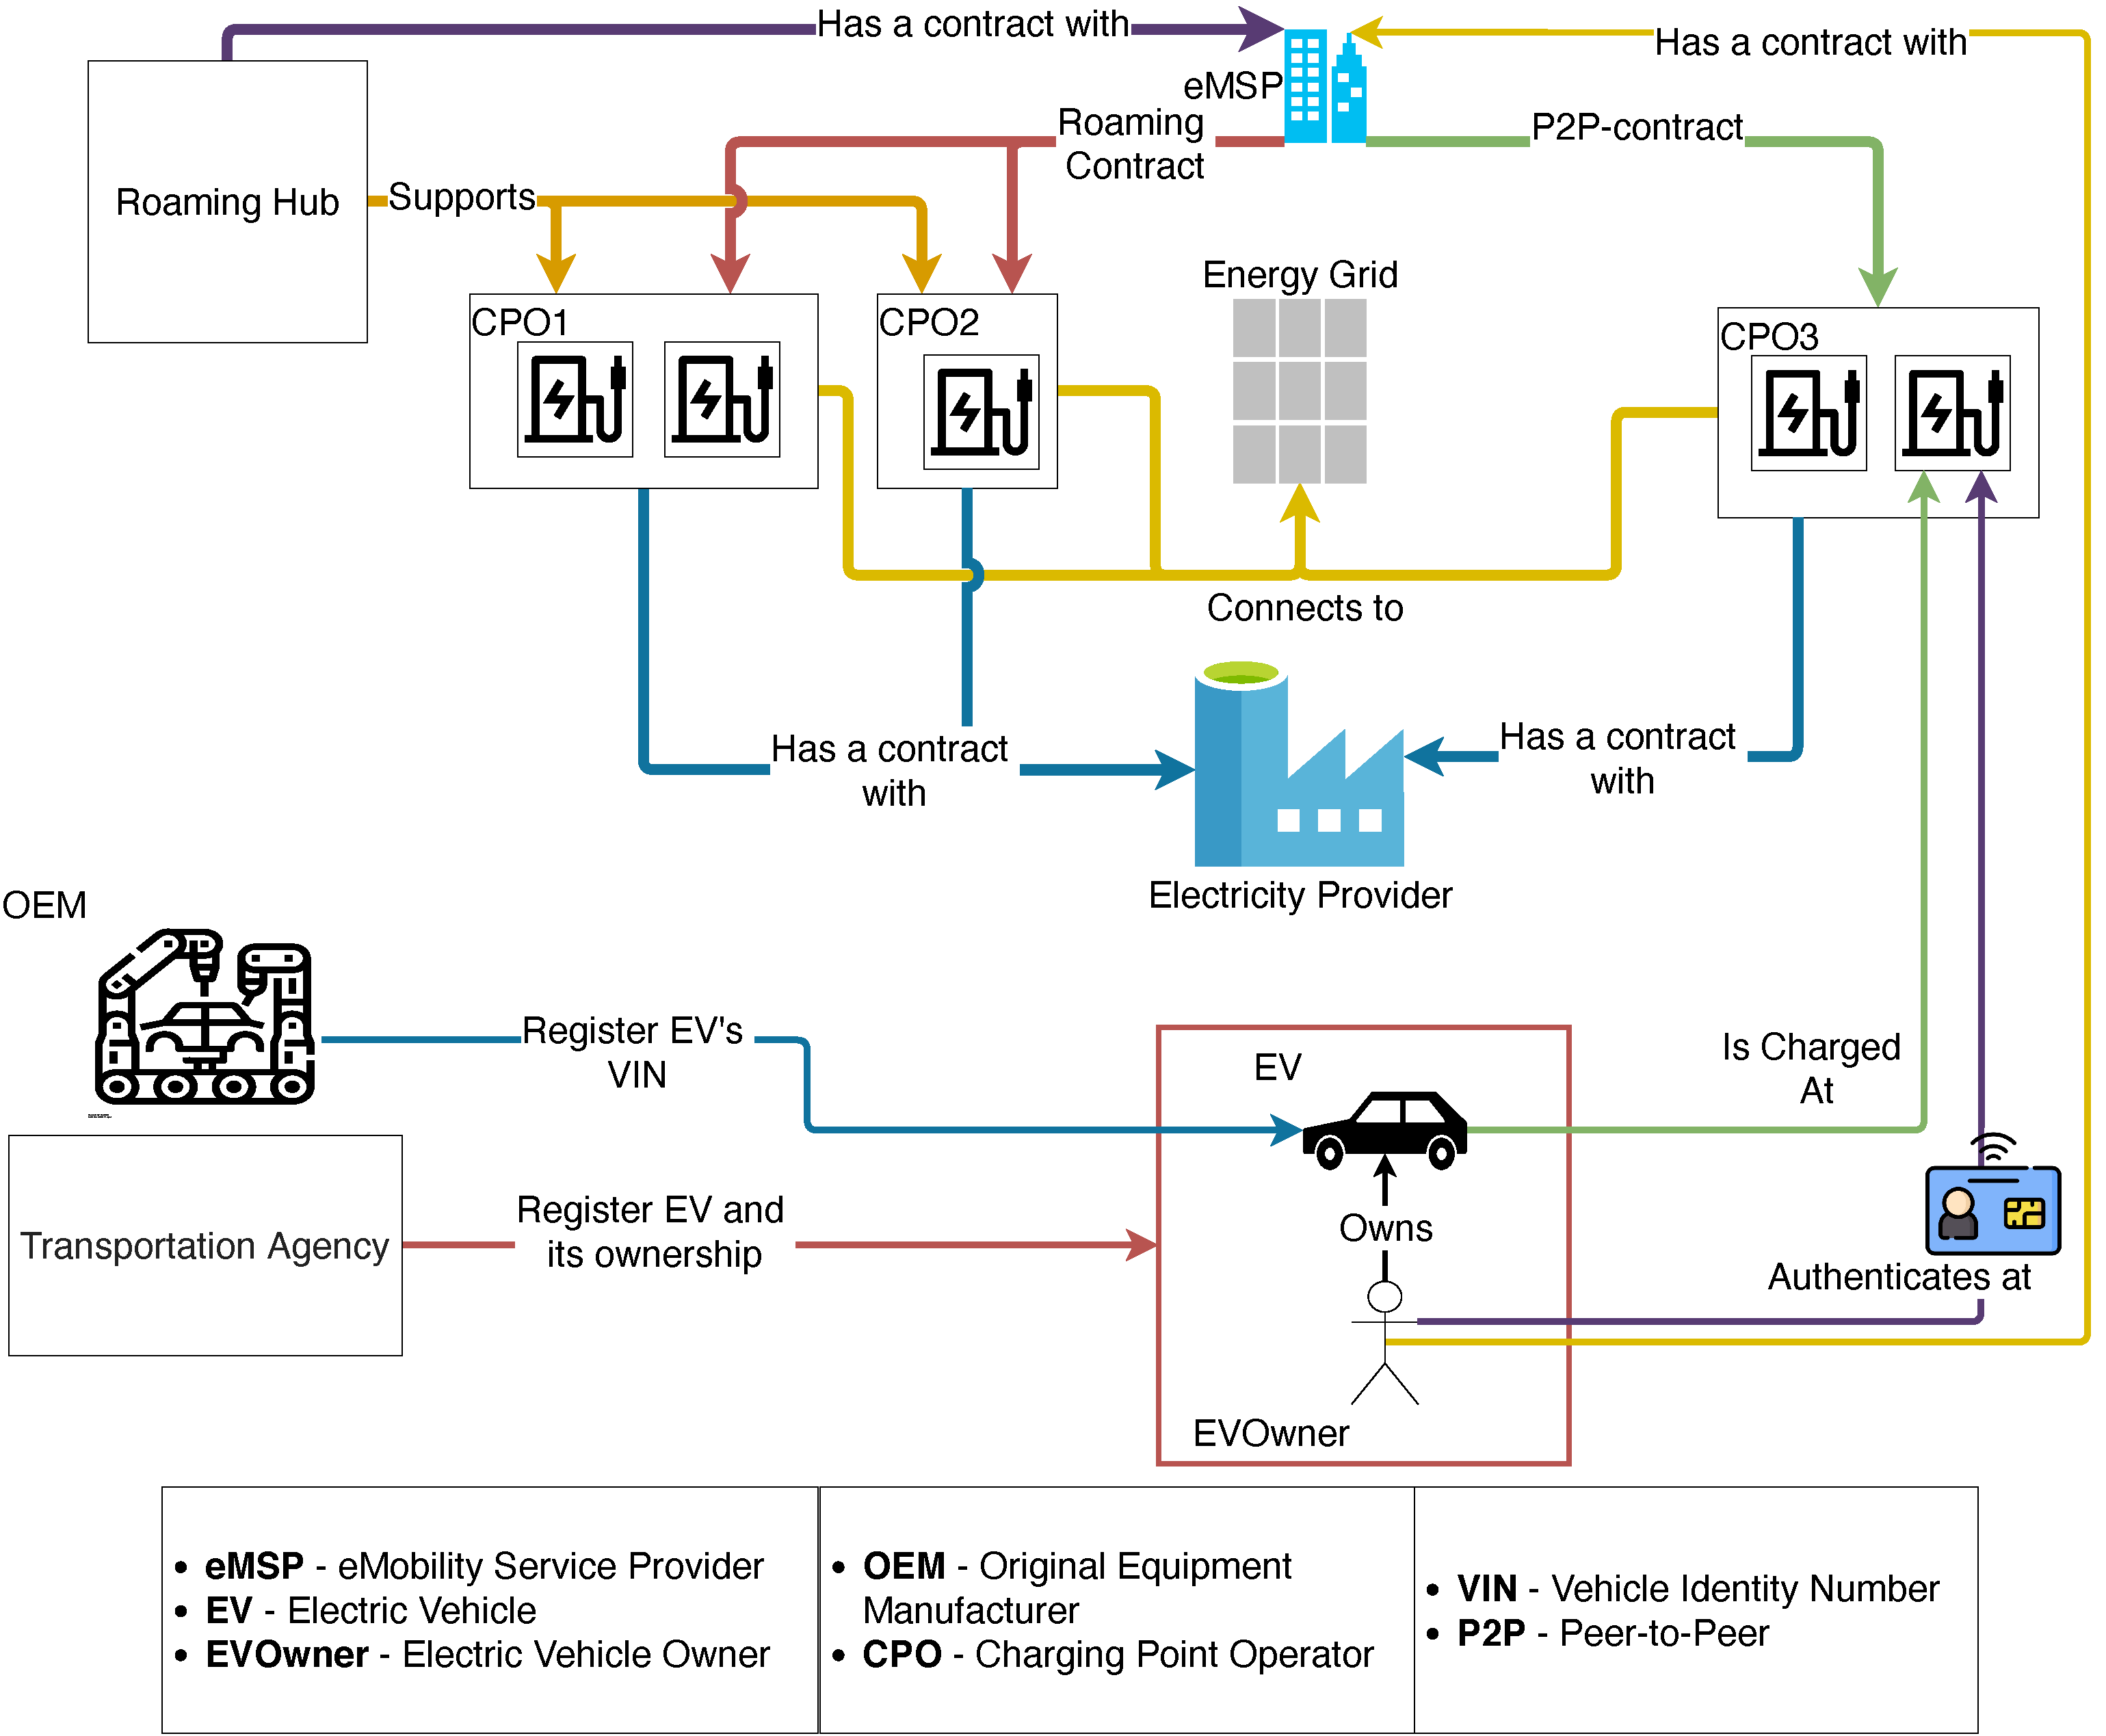
\includegraphics[width=0.85\linewidth]{images/Initial_model.pdf}
    \caption{High-level overview of Case Study}
    \label{fig:High-level overview}
\end{figure}

\subsubsection{Users and Information Flows}
\label{subsubsec:users_and_information_flows}

The diagram presented in Figure~\ref{fig:High-level overview} displays the parties that are involved in this case study, and how these connect between each other. The system comprises of three distinct flows: the "Service Providers", the "EV Owner and EV Interactions" and at last the "Charging and Billing".

\paragraph{Service Providers}

The primary party in this flow is an \acrfull{eMSP}, whose main goal is to provide the largest network of charging points available to its clients, the \glspl{EV Owner}. If an EV Owner wishes to charge their EV, there is the need to sign a contract with an eMSP (\textcolor{yellow}{Thin Yellow Line}).

In order to expand the network, the eMSP company may hire subsidiaries whose role is to act as a \acrfull{CPO}. These CPOs may have a Peer-to-Peer contract (\textcolor{green}{\textbf{Bold Green Line}}) or be part of Roaming Hubs of the company (\textcolor{purple}{\textbf{Bold Purple Line}}) and have a Roaming Contract (\textcolor{red}{\textbf{Bold Red Line}}). The CPOs are the ones that own the \glspl{CS} and are responsible for guaranteeing their good functioning. 
The CPOs are the ones who negotiate with the \glspl{EP} directly to obtain electricity for the Charging Stations (\textcolor{blue}{\textbf{Bold Blue Line}}). Additionally, the CPOs are the ones who directly communicate with the Energy Grid if one is to consider bilateral communication to balance the grid (Vehicle-To-Grid) (\textcolor{yellow}{\textbf{Bold Yellow Line}}).

In some occasions the eMSPs may have a preferred CPO contract, which in turn provides a cheaper price for EV Owners. In the occasion where the EV Owner tries to charge the vehicle in a different CPO (who also has a contract with the same eMSP), the fee may be larger. This also addresses another important point: when an EV Owner charges the EV at a new CPO, the CPO will not have the user credentials ready for authentication. When this happens the CPO may directly connect to the eMSP looking to authenticate the user; if this fails, the Roaming Hub will act as an intermediary between CPOs and eMSPs, in order to provide an alternative authentication route. Whenever an EV Owner wishes to charge their EV, the Roaming Hub will check whether the user has been authenticated in one of the other CPOs in the Hub. This has an associated cost, since reaching to more parties means taking a longer authentication route.

\paragraph{EV Owner and EV Interactions}

In order for an EV to be driven by someone, it requires documentation to attest a vehicle's unique identifier, which is named \acrfull{VIN} and may be contained in a \acrfull{VBC}, and whose issuer is the respective \acrfull{OEM} (\textcolor{blue}{Thin Blue Lines}).

For someone to charge their vehicle they must be the owners of said vehicle\footnote{This is a simplifying assumption for the purposes of this work and in reality this assumption does not always hold (e.g. when lending the vehicle to a relative, or when being the owner of a vehicle rental agency, more on this will be covered in the evaluation chapter)}. This means that the EV Owner and the EV must be registered together in the \acrfull{TA} of the respective country (RDW or "Rijksdienst voor het Wegverkeer" in the Netherlands) so that an EV Owner is legally allowed to drive their EV on the roads (\textcolor{red}{Thin Red Lines}).

\paragraph{Charging and Billing}

After the contract with the eMSP is signed (as mentioned in the "Service Providers" flow), the EV Owner may charge the EV at any of the CSs offered by CPOs who are contracted by the same eMSP. This requires the EV Owner to authenticate at the CSs using smart cards or login credentials on a mobile app provided by the eMSP for NFC authentication (\textcolor{purple}{Thin Purple Line}). Only if the authentication succeeds, the CS will start powering the EV (\textcolor{green}{Thin Green Line}). If an EV Owner tries to charge the EV at a CPO that does not have a contract with its eMSP, the charging is not possible.

The current system architecture's billing system comprises of the EV Owner making a monthly payment to the eMSP with the total of the expenses for the charging transactions in that given month. The CPOs obtain their profits from reselling the energy from the Electricity Providers to the EV Owners and also through a fees-model paid by the eMSP which is directly related to the number of EVs charging at the CPOs Charging Stations. The Roaming Hubs profit from providing an authentication route to the eMSPs, in case the CPOs have no past record of the user in the system. The EPs make profit from selling the energy directly to the CPOs with whom they have a contract.


\subsubsection{Current Liabilities}
\label{subsubsec:current_liabities}

In the current implementation of the Electric Vehicle Charging system, there are some liabilities which have been extracted based on the input provided by the domain experts. These include problems of transparency, security, data privacy and functionality.

\begin{itemize}
    \item The EV Owners are not aware of the price rate of the kWh at the time of charging, and are only aware of the total expense of one transaction when it is described in the monthly invoice. Consequently, CPOs have the chance to boost rates and the price of the energy sold to the EV Owners since the rates are not presented to the EV Owners before charging.
    \item Problems with current authentication is leading to identity fraud. With the usage of smart cards there is the chance for these to be cloned and used by malicious entities. With the usage of login credentials there is the problem with account hijacking which also leads to identity theft. Reports have been made for multiple charging sessions taking place far apart at close times, under the same identity.
    \item Still regarding authentication, in the current architecture the CPOs will try to authenticate the EV Owners by going directly to the eMSPs. If something goes wrong in this communication (e.g. fault in the network), and if the CPOs are contained within a Roaming Hub, they have the option to authenticate the EV Owners by means of those Roaming Hubs. When this occurs both CPOs and eMSPs are at a loss, given that the revenue is reduced by the introduction of a new party in this transaction (the Roaming Hub).
\end{itemize}

\subsection{List of requirements}
\label{subsec:list_of_requirements_and_decisions}

When designing a possible novel architecture, it is important to consider the current limitations in the field of SSI with IoT, and understand which technologies have the power to mitigate or erase such constraints. Also, given the current system architecture for the Charging of EVs, the requirements for that system should also be accounted for in a new architecture. Following the diagram presented in Figure~\ref{fig:High-level overview} which depicts an overview of the current system architecture, the requirements for a new architecture will be listed, followed by the respective rationales.

\subsubsection{Key Drivers}
\label{subsubsec:key_drivers}

In order to extract the key drivers of this system, an analysis on the literature was made in Section~\ref{subsubsec:Blockchain-based_SSI_with_IoT} to understand which are the most analyzed quality attributes when assessing SSI alone or together with its integration with IoT.

\paragraph{Scalability}

The literature highlighted as an urgent need that an SSI-based solution for IoT devices has the possibility to scale as the number of connected devices grow \cite{luecking2020decentralized} \cite{zhu2018identity} \cite{lo2019analysis} \cite{zhu2017autonomic}. The reason is evident, as mentioned in the introduction, the number of IoT devices is expanding and the need for a scalable IdMS is extremely important.

\paragraph{Performance}

Another important aspect to consider is the performance of the network. If the network contains low throughput, the number of \acrfull{TPS} may not satisfy the high volume of data collected by IoT devices \cite{lo2019analysis}. 

\paragraph{Security and Privacy}

Matters of data privacy, security and tampering are some of other aspects which need to be accounted when dealing with massive quantities of data and the identity of billions of IoT devices \cite{luecking2020decentralized} \cite{zhu2018identity} \cite{s18082575} \cite{theodouli2020towards}. These were matters addressed in literature which focused on an IdMS solution for IoT, which demonstrated to be sufficiently supported by blockchain solutions \cite{lo2019analysis}.

\paragraph{Other Relevant Quality Attributes}

While not key drivers, other quality attributes that were mentioned in the literature should also be taken into account when designing a new system architecture. Interoperability \cite{luecking2020decentralized} \cite{zhu2018identity} and availability \cite{theodouli2020towards} are examples of other NFRs which will also be considered in the selection of the components of the new systems architecture.

Regarding the availability of the system, according to Transport \& Environment, Europe's leading clean transport campaign group, a system whose goal is to provide electric vehicle charging stations to clients requires a 97\% uptime guarantee, according to the latest published report \cite{todts_2020}.

\subsubsection{Functional Requirements}

The \glspl{FR} displayed in Table~\ref{tab:functional_requirements} relate to the technical functionality of the Electric Vehicle Charging system, and are organized to better display what each functionality will add to the system. The requirements have been categorized using the MoSCoW prioritization technique\footnote{\url{https://www.productplan.com/glossary/moscow-prioritization/}}, where each requirement is tagged with one of the following levels of priority: "Must have", "Should have, "Could have" and "Will not have".

\begin{longtable}{|p{.1\textwidth}p{.15\textwidth}p{.70\textwidth}|}
    \hline
    \textbf{ID} & \textbf{Priority} & \textbf{Requirement}\\
    \hline
    \hline
   \textbf{FR-1.1} & Must & \textit{The system must allow for an EV Owner to charge its EV at a CS}\\
   \textbf{FR-1.2} & Should & \textit{The rate at which the kWh is being sold to the EV Owner should be presented before the charging starts}\\
   \textbf{FR-1.3} & Must & \textit{The EV Owner must be prompted to accept/reject the price of the kWh}\\
   \textbf{FR-1.4} & Could & \textit{At the end of a transaction, the EV Owner could receive proof of the transaction with the amount due}\\
   \hline
   \textbf{FR-2.1} & Must & \textit{A CS must belong to a CPO}\\
   \textbf{FR-2.2} & Must & \textit{A CPO must have a contract with an eMSP}\\
   \textbf{FR-2.3} & Must & \textit{A CPO must have a contract with an EP to provide power to its Charging Stations}\\
   \hline
   \textbf{FR-3.1} & Should & \textit{EV Owners should prove they are the owners of their EV to a CS}\\
   \textbf{FR-3.2} & Must & \textit{EV Owners must attest they have a valid contract with an eMSP that the CS's CPO has a contract with}\\
   \textbf{FR-3.3} & Could & \textit{An EV Owner could be made aware that the CS belongs to the CPO it claims} \\
   \textbf{FR-3.4} & Should & \textit{The process of setting up the connection and verifying credentials should be executed with the least EV Owner intervention as possible.}\\
   \hline
   \textbf{FR-4.1} & Must & \textit{An EV and the information regarding its EV Owner must be registered with the TA in order for the EV to be on the roads and to be charged at a CS}\\
   \hline
   \textbf{FR-5.1} & Must & \textit{The system must not write \acrfull{PII} in a publicly accessible data repository}\\
   \textbf{FR-5.2} & Must & \textit{Every credential issued must be verifiable using cryptographic proof}\\
   \hline
   \textbf{FR-6.1} & Must & \textit{An EV Owner must be able to delegate (temporary) possession of its EV to another driver}\\
   \hline
    \caption{Functional Requirements}
    \label{tab:functional_requirements}
\end{longtable}
    
\subsubsection{Non-Functional Requirements}

The \glspl{NFR} presented in this section are closely related to the key drivers identified in Section~\ref{subsubsec:key_drivers}. The key drivers act as important guidelines in the development of the system. The system-to-be aims to achieve the desired key attributes by fulfilling the non-functional requirements mentioned in Table~\ref{tab:non-functional_requirements}. The requirements have been categorized using the MoSCoW prioritization technique \footnote{\url{https://www.productplan.com/glossary/moscow-prioritization/}}, where each requirement is tagged with one of the following levels of priority: "Must have", "Should have, "Could have" and "Will not have". 
Each set of requirements directly links to a key driver according to the following match: 

\begin{itemize}
    \item \textbf{NFR-1.X} - Scalability
    \item \textbf{NFR-2.X} - Performance
    \item \textbf{NFR-3.X} - Security and Privacy
    \item \textbf{NFR-4.X} - Other Relevant Quality Attributes
\end{itemize}

\begin{longtable}{|p{.1\textwidth}p{.15\textwidth}p{.70\textwidth}|}
        \hline
        \textbf{ID} & \textbf{Priority} & \textbf{Requirement}\\
        \hline
        \hline
       \textbf{NFR-1.1} & Must & \textit{The system must scale according to the growth of the market. Supposing an adoption in the Dutch Market (300k EVs in 2020 \protect\footnotemark)     \footnotetext{\url{https://www.rvo.nl/sites/default/files/2020/11/Statistics\%20Electric\%20Vehicles\%20and\%20Charging\%20in\%20The\%20Netherlands\%20up\%20to\%20and\%20including\%20October\%202020\%20-\%202.pdf}}, the system must be able to support this number of vehicles and the estimated growth (3M EVs by 2030 \protect\footnotemark) 
       \footnotetext{\url{nklnederland.com/news/sparkcity-3-million-evs-by-2030-2/}}}\\
       \hline
       \textbf{NFR-2.1} & Should & \textit{The system should be able to kickstart the charging process in a reasonable amount of time (no longer than the time required without VCs, less than 1 minute)}\\
       \textbf{NFR-2.2} & Must & \textit{The system must withstand multiple users accessing the system at the same time, with no loss of information}\\
       \textbf{NFR-2.3} & Must & \textit{The user must be presented with information on how to engage with the CS in less than 5 seconds}\\
       \textbf{NFR-2.4} & Should & \textit{The process of validation the client's credentials should not take longer than the original method (designed for 2 seconds, with the worst case scenario being 30 seconds)}\\
       \hline
       \textbf{NFR-3.1} & Should & \textit{The system should be constantly updated to mitigate the risk of quantum-attacks, by employing state-of-the art cryptography}\\
      \textbf{NFR-3.2} & Must & \textit{The system must comply with Dutch regulations, including \acrfull{GDPR}}\\
      \textbf{NFR-3.3} & Must & \textit{The system must be protected against forgery of identity, so that in the case of theft of identity the malicious party cannot use the system}\\
      \hline
      \textbf{NFR-4.1} & Must & \textit{A CS must have an active internet connection to authenticate the EV Owner}\\
      \textbf{NFR-4.2} & Must & \textit{The systems implementation must allow for as many agent implementations as possible, opting for solutions that favor interoperability}\\
      \textbf{NFR-4.3} & Must & \textit{The system must offer a 97\% uptime guarantee \cite{todts_2020}} \\
      \hline
\caption{Non-Functional Requirements}
\label{tab:non-functional_requirements}
\end{longtable}